% **************************************************************************** %
\chapter{Benutzerhandbuch}
\label{chap:userguide}
% **************************************************************************** %

\noindent\adjustbox{valign=t}{\begin{minipage}{44mm}
    
\includegraphics[width=29mm]{images/userguide/danger.png}\footnotemark
\end{minipage}}
\noindent\adjustbox{valign=t}{\begin{minipage}{95mm}
    Wichtiger    Hinweis: Die    Installation    und    Inbetriebnahme    darf
    ausschliesslich  durch  eine  autorisierte  Elektrofachkraft  ausgef\"uhrt
    werden. Bei der  Installation des Systems  ist zwingend zu  beachten, dass
    Teile  der Photovoltaikanlage  st\"andig unter  Spannung stehen  k\"onnen,
    auch bei abgeschalteter Anlage.
\end{minipage}}
\footnotetext{
    Bildquelle: \cite{ref:danger}
}

% ---------------------------------------------------------------------------- %
\section{Installation und Inbetriebnahme}
\label{sec:userguide:installation}
% ---------------------------------------------------------------------------- %

Die Installation des Master-Ger\"ates erfolgt im Generatoranschlusskasten. Das
Master-Geh\"ause  wird  auf  einer  Hutschiene  platziert  und  innerhalb  des
GAKs  mit  \SI{230}{\volt}  AC  gespeist. Die DC-Leitungen  von  bis  zu  drei
Str\"angen pro  \Master~ werden auf die  daf\"ur vorgesehenen Anschlussklemmen
gef\"uhrt. Der   maximale    Leiterquerschnitt   der    DC-Leitung   betr\"agt
\SI{4}{\milli\meter\squared}  und  ist   f\"ur  g\"angige  Photovoltaikanlagen
ausreichend.

Um eine  einwandfreie Alarmierung im  Fehlerfall zu gew\"ahrleisten,  wird die
Installation  mindestens eines  externen  Meldeger\"ats empfohlen. \"Uber  die
beiden Relaiskontakte  am Master-Ger\"at  k\"onnen externe Ger\"ate  mit einer
Nennspannung bis max. \SI{250}{\volt} \todo{korrekt?} geschaltet werden.

Nach der  Installation und dem  Einschalten des Master-Ger\"ates   erfolgt die
Installation  der Sensorkomponenten. Jedes  PV-Modul  wird im    zugeh\"origen
Anschlusskasten  mit einem  Sensor  ausgestattet. Der Sensor  wird \"uber  die
beiden  Kupferdr\"ahte  der  Platine  an den  Anschlussklemmen  des  PV-Moduls
angeschlossen. Dabei  ist die  richtige  Polarit\"at  zu beachten. Sobald  der
Sensor mit der DC Leitung verbunden ist, wird die Seriennummer automatisch vom
Master-Ger\"at erfasst  und ins System integriert. Jeder  Sensor besitzt dabei
eine einzigartige  Seriennummer. Diese Seriennummer wird  jeweils zus\"atzlich
in  Form eines  Klebstreifens  mit dem  Sensor  mitgeliefert. Um den  Standort
jedes  Sensors  zu dokumentieren,  sind  die  Klebstreifen im  Anlageplan  auf
dem  jeweiligen Modul  aufzutragen. Gleiches Vorgehen  f\"ur die  Installation
weiterer Sensoren.   Ist ein  Sensor defekt, kann  die gesamte  Platine bequem
ausgetauscht  werden. Die   neue  Seriennummer  wird  dabei   automatisch  vom
Master-Ger\"at erfasst und ins System  integriert. Dabei ist zu beachten, dass
der Anlageplan mit den Seriennummern-Klebstreifen stets angepasst wird.


% ---------------------------------------------------------------------------- %
\section{Regul\"arer Betrieb}
\label{sec:userguide:regular}
% ---------------------------------------------------------------------------- %

S\"amtliche  Einstellungen des  Systems  werden \"uber  das Touch-Display  des
Master-Ger\"ates get\"atigt. Im regul\"aren Betrieb sind \"ublicherweise keine
Einstellungen vorzunehmen. Der  Gr\"une Knopf,  rechts vom Display,  dient zum
Aus- bzw. Einschalten  des Displays. Im regul\"aren Betrieb  empfiehlt es sich
jedoch aus energietechnischen Gr\"unden das Display ausgeschaltet zu lassen.

\begin{wrapfigure}{r}{0.45\textwidth}
    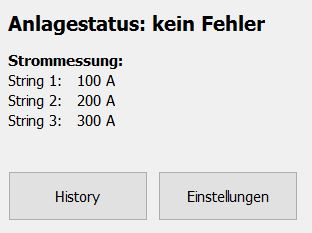
\includegraphics[width=0.45\textwidth]{images/userguide/screen0.png}
    \caption{Hauptmenu}
    \label{fig:userguide:screen0}
\end{wrapfigure}

Bei Bet\"atigung des gr\"unen Knopfes  erscheint das Hauptmenu, dargestellt in
Abbildung \ref{fig:userguide:screen0}. Dieses dient  einerseits zur Auflistung
aktueller  Messwerte der  Strangstr\"ome  und  des Anlagestatus,  andererseits
f\"uhrt  es mittels  weiterer  Buttons in  die  jeweiligen Untermenus. In  der
obersten Zeile  \emph{Anlagestatus} wird  dargestellt, ob  ein Problem  an der
Anlage vorliegt. Wird bei Anlagestatus  \emph{kein Fehler} angezeigt, liegt an
der  Anlage keine  St\"orung vor. Wird  jedoch die  Fehlfunktion eines  Moduls
detektiert, erfolgt eine Meldung im Hauptmenu. (Weiter Infos zum St\"orbetrieb
im Kapitel weiter unten).

\vspace*{3em}
\noindent\adjustbox{valign=t}{\begin{minipage}{0.475\textwidth}
    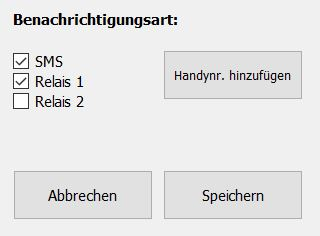
\includegraphics[width=\textwidth]{images/userguide/screen1.png}
    \figcaption[Master: Menu: Einstellungen]{Einstellungen}
    \label{fig:userguide:screen1}
\end{minipage}}
\noindent\adjustbox{valign=t}{\begin{minipage}{0.475\textwidth}
    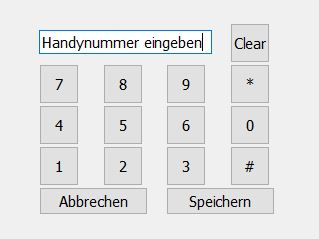
\includegraphics[width=\textwidth]{images/userguide/screen2.png}
    \figcaption[Master: Menu: Einstellungen: Telefonnummer]{Eingabe einer Telefonnummer}
    \label{fig:userguide:screen2}
\end{minipage}}

Im     Untermenu     \emph{Einstellungen},    dargestellt     in     Abbildung
\ref{fig:userguide:screen1},   k\"onnen  die   SMS-Benachrichtigung  und   die
Relaisausg\"ange konfiguriert werden. Beim  Hinzuf\"ugen einer Handynummer mit
korrekter Vorwahl  (Bsp. \code{0041 79  612 33  22}) und bei  Bet\"atigung des
entsprechenden K\"astchens   wird automatisch die Benachrichtigung  \"uber SMS
aktiviert. Das zugeh\"orige Menu  ist in Abbildung \ref{fig:userguide:screen2}
gezeigt. Wie auch die beiden Relais 1 und Relais 2 werden bei der Bet\"atigung
des jeweiligen K\"astchens aktiviert. \"Uber den Button \emph{Speichern} werden
die Einstellungen im System \"ubernommen.


% ---------------------------------------------------------------------------- %
\section{St\"orbetrieb}
\label{sec:userguide:errors}
% ---------------------------------------------------------------------------- %

Wird die Fehlfunktion eines  Moduls detektiert, erfolgt eine St\"orungsmeldung
an das  Master-Ger\"at. Folglich erscheint  im Hauptmenu  des Master-Ger\"ates
die  Seriennummer des  entsprechenden Moduls  wie auch  Datum und  Uhrzeit der
Fehlererkennung, wie in Abbildung \ref{fig:userguide:screen3} gezeigt.

Zeitgleich  werden  am  Master-Ger\"at  zwei  Relaiskontakte  bet\"atigt,  die
f\"ur externe  akustische oder  optische Meldeger\"ate  vorgesehen sind. Diese
externen Meldeger\"ate lassen sich mit  dem entsprechenden Button im Hauptmenu
quittieren. Sofern  unter  \emph{Einstellungen}  eine  Handynummer  hinterlegt
wurde, erfolgt  zus\"atzlich eine Fehlerbenachrichtigung an  das entsprechende
Mobiltelefon.

Um die Energieverluste zu minimieren, sollte bei einem Fehlerfall umgehend ein
Installateur der Photovoltaikanlage konsultiert werden. Sobald das fehlerhafte
Modul wieder einwandfrei funktioniert, wird die Fehlermeldung im Hauptmenu des
Master-Ger\"ates  automatisch ausgeblendet. Im  Untermenu \emph{Fehlerverlauf}
(Abbildung  \ref{fig:userguide:screen4} sind  alle bisherigen  Fehlermeldungen
der Anlage ersichtlich.

\vspace*{3em}
\noindent\adjustbox{valign=t}{\begin{minipage}{0.475\textwidth}
    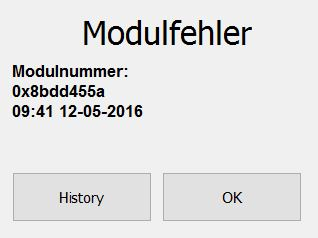
\includegraphics[width=\textwidth]{images/userguide/screen3.png}
    \figcaption[Master: Menu: Modulfehler]{Fehler bei einem Modul}
    \label{fig:userguide:screen3}
\end{minipage}}
\noindent\adjustbox{valign=t}{\begin{minipage}{0.475\textwidth}
    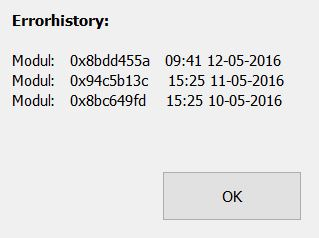
\includegraphics[width=\textwidth]{images/userguide/screen4.png}
    \figcaption[Master: Menu: Einstellungen: Fehlerverlauf]{Fehlerverlauf der Anlage}
    \label{fig:userguide:screen4}
\end{minipage}}
